\section{Introduction}

% General paragraph on AD
Alzheimer's Disease (AD) is a neurodegenerative disease that causes progressive cognitive impairment, leading to death \cite{Lane2018}. AD has currently no cure and puts a strong strain in healthcare systems, due to the care needed by patients at later stages of the disease \cite{AlzheimersAssociation}. AD is a multifactorial disease that affects different systems and processes of the brain \cite{Jack2010}. Those processes are captured using different biomarkers coming from various imaging modalities, such as magnetic resonance imaging (MRI) to capture atrophy or positron emission tomography (PET) for glucose uptake or blood flow. For a disease as complex as AD, it is necessary to study not only how those different biomarkers interact between each other, but also their evolution. For this reason, the use of longitudinal data, e.g., data captured over several time points, is extremely valuable to researchers. However, it is often difficult to use this kind of medical data, as it can present problems of data missingness across modalities (due to invasive acquisition methods, such as lumbar puncture for cerebrospinal fluid acquisition) and across time (due to medical follow-ups that were missed, for example). \\

% Introduction to disease progression methods (probably would be removed in a journal paper).
Modelling longitudinal, multivariate data is a difficult task \cite{Verbeke2014}. For neurodegenerative diseases, disease progression modelling methods can be used to leverage these medical data and find and predict the trajectories of biomarkers, which could lead to better characterization and understandanding on how the the evolution of the disease over time. Such techniques have been used in many degenerative diseases, including AD \cite{Oxtoby2017,Marti-Juan2020}. Examples of those techniques include event-based models \cite{Young2014,Young2015a,Fonteijn2012}, which discover, for a set of biomarkers, the order in which they will degenerate over the disease progression; Gaussian processes \cite{Lorenzi2015b,Hyun2016,Lorenzi2019} which allow to characterize the uncertainty of the progression; among other types of methodologies \cite{Marinescu2019, Young2017}. These methods, however, are usually limited in the number of modalities they can combine (sometimes only one or two) or in the amount of longitudinal data they use (cross-sectional data, or only short-term data). Moreover, it is not clear how to combine longitudinal modalities with non-temporal ones, such as demographic or genetic data, which can influence the trajectory of the disease. More recently, Antelmi et al. \cite{Antelmi2019} proposed a generative method based on variational auto encoders (VAE) using multiple channels or modalities of cross-sectional data. Their method inferred a lower dimensional latent space generated jointly from all the modalities, and modelled the dependence across modalities, being able to generate missing modalities for specific patients. \\

% need to introduce Cao2019 (is the CCA paper, already in bib)
For sequence learning, recurrent neural networks (RNN) \cite{Hochreiter1997} have become a powerful tool. Although they have been mainly used for natural language processing \cite{Goldberg2017}, they have also been used for sequence modelling in other fields, like image generation \cite{Gregor2015a}, and including AD disease progression \cite{Wang2018,Ghazi2019}. Variational recurrent neural networks \cite{Chung2015,Fabius2015} add a variational layer to the RNN arquitecture, allowing it to capture more complex temporal variation by setting temporal dependencies between the random latent variables. Outside RNNs, Cao et al. \cite{Cao2019} recently proposed a method using canonical correlation analysis to compare two different time series, applied to functional MRI analysis. \\ 

In this chapter, we propose a multi-channel recurrent variational method for disease progression. Similarly to \cite{Antelmi2019}, we jointly model the dependencies across channels and the temporal dependencies for each channel, but adding a variational recurrent block to capture temporal dependencies alongside every channel. The model is able to use longitudinal data with variable number of time points and missing modalities. We show that the model captures the progression of the disease and the relationships between the modalities. We show the capability of our model to both predict missing modalities from existing ones and predict future timepoints. The results show in this chapter are preliminary at the time of writing this thesis, and more research is being conducted to improve upon them. \\

%% Needs to be updated when the whole chapter is detailed
The chapter is organized as follows: In Section \ref{rnn:background}, we explain the background on the methods used in the chapter: recurrent neural networks and variational autoencoders. In Section \ref{rnn:methods} we detail the propose method, derive the variational lower bound used to optimize the model, and detail the experiments conducted, as well the data used. Section \ref{rnn:results} contains the detailed results of our experiments. In Section \ref{rnn:discussion} we discuss the current results and show the most important contribution. Finally, in Section \ref{rnn:conclusions} we summarize the chapter, address the limitations of our model, and propose future lines of research.

\section{Background}
\label{rnn:background}
Before introducing the proposed method, we briefly describe the basics of the two groups of methods we use: recurrent neural networks and variational autoencoders.

\subsection{Recurrent Neural Networks}
%% Have to do the figure

RRNs are able to model sequences by recursively processing the data, using previous outputs as inputs, while maintaining a hidden state $h$, a variable that can store information of the sequence. This makes this type of network ideal for temporal sequences. A basic RNN architecture can be described as:

\begin{equation}
    h_t = \mathit{\sigma}(W_h h_{t-1} + W_x x_{t} + b_h),
    %& y_t = \mathit{\sigma_y}(W_y h_t + b_y),
\end{equation}

where $x_t$ is the vector of data at time $t$ and $h_{t}$ is the hidden state of the recurrent network at time $t$. $\sigma$ is a non-linearity, while $W$ and $b$ are the weights and biases of the unit. RNN are recurrent networks in the sense that each subsequent state $h_t$ depend on all the previous ones. Figure \ref{fig:rnnvae:rnn} shows this recurrence and how it unrolls for a single RNN for an input sequence $x = (x_0,x_1, ..., x_t)$. \\

\begin{figure}[!htbp]
  \centering
  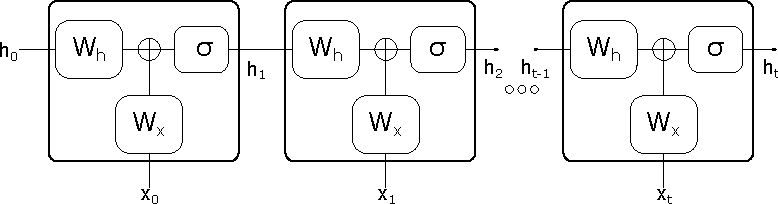
\includegraphics[width=0.9\textwidth]{figures/rnnvae/rnn-fig.pdf}
  \caption[Unroll of the recurrency for a basic RNN.]{Unroll of the recurrency for a simple RNN and input sequence $x = (x_0,x_1, ..., x_t)$. $W_h$ and $W_x$ are weight matrices. Biases not shown in the figure.}\label{fig:rnnvae:rnn}
\end{figure}

This is the basic formulation of a RNN, and while it works well for short-range sequences, it can fail for longer sequences due to gradient vanishing \cite{Hochreiter1998}, caused by the large number of operations needed to compute the gradient during training. More complex formulations have been proposed in the literature to address those issues, such as LSTM \cite{Hochreiter1997} or GRU \cite{Chung2014}. For a more in depth look at RNNs, including training, formulation and derivation, we refer the reader to \cite{Sherstinsky2020}.  \\

\subsection{Variational Autoencoders}

Variational autoencoders (VAE) are probabilistic models that encode the observed input $x$ into a vector of latent random variables $z$, creating a low-dimensional latent space that capture the main variations of the input space and allow for sampling and inference. The joint probability of a standard VAE is:

\begin{equation}
    p(x,z) = p(x|z)p(z),
\end{equation}

where $p(x|z)$ is the likelihood of the input data conditioned on $z$, while $p(z)$ is the prior distribution of the latent variable. We want to infer the posterior $p(z|x)$, which will give us the best $z$ distribution for our data:

\begin{equation} \label{eq:rnnvae:intract}
\begin{split}
p(z|x) = \frac{p(x,z)}{p(x)}, \\
\text{with } p(x) = \int p(x,z) dz
\end{split}
\end{equation}

However, this posterior is usually intractable. In Equation \ref{eq:rnnvae:intract}, $p(x)$ is intractable for more complex distributions. To solve this, we perform variational inference by approximating another distribution to the real posterior. We call this approximate posterior $q(z|x)$. We can use a lower bound on the distribution of $x$ to define an optimization objective that is tractable: 

\begin{equation}
    log p(x) \geq \mathbb{E}_{q(z|x)} log(p(x|z)) - \mathcal{D}_{KL}(q(z|x)|p(z)),
\end{equation}

where $D_{KL}$ is the Kullback-Leibler (KL) divergence between two distributions. The full derivation of this lower bound can be found on \cite{Kingma2014}. The first term of this lower bound is the reconstruction error, and tries to maximize the similarity between the original and reconstructed data, while the second term is the regularization term, and represents the divergence between the encoder and the prior of the latent space (usually a Normal distribution). This term forces the latent distribution not to directly encode an identity between input and output. \\

Variational auto-encoders can be parametrized by defining $p(x|z)$ and $q(z|x)$ as neural networks (usually called the decoder and the encoder, respectively), and we can train their associated parameters using gradient descent by maximizing the lower bound. However, directly sampling from the encoder $z~q(z|x)$ lead to high variance estimates of the gradient, and makes training very difficult. To solve this, Kingma et al. \cite{Kingma2015} proposed to reparametrize the estimation by introducing a random variable from a simple distribution $\varepsilon ~ N(0,1)$ and mapping it to z. For example, if q(z|x) is parametrized as a Normal distribution $\mathcal{N}(\mu, \sigma)$:

\begin{equation}
\begin{split}
    \varepsilon \sim \mathcal{N}(0,1) \\
    z = \mu + \sigma \varepsilon
\end{split}
\end{equation}

This approach leads to a lower variance estimator and allows for a smooth training.

\section{Methods}
\label{rnn:methods}

\subsection{Recurrent multi-channel variational auto-encoder}
% Metode

% T can be variable across channels. Should I put this?
Let $x = (x^0,...,x^c,...,x^{C-1})$ be a set of data sequences across $C$ different channels. Each of these sequences are defined over $T$ timepoints  $x^c = (x^c_{0},...,x^c_{t},...,x^c_{T-1})$. We base our model on two assumptions: the existence of temporal dependencies across time-steps for each different channel $x^c$, and there are cross-channel dependencies, each describing a part of an underlying joint trajectory of the disease. To capture dependencies on the data across time, we define a model using a variational RNN, similar to the one described in \cite{Chung2015}, where we generate latent variables $z_t$ at each timestep $t$, which are conditioned on the hidden states of the RNN of every channel at the previous temporal step $h_{t-1}$. For the inter-channel dependencies, we assume, we similarly to \cite{Antelmi2019}, that each channel $x^c$ share the same latent space $z$, and that each channel is conditionally independent from the others. \\

We first describe the encoder and the decoder of the variational autoencoder for a specific channel $c$ and timepoint $t$:

\begin{equation} 
\begin{aligned} \label{rnn:eq:generative}
\displaystyle
& \mathit{p}(x^c_t | z_{\leq t}, x^c_{< t}) \sim \mathcal{N}(\mu_{x^c_t},\sigma_{x^c_t}), \text{ where } \mu_{x^c_t},\sigma_{x^c_t} = \varphi_{dec}(\varphi_{z}(z_t), h^c_{t-1}) \\
& \mathit{q}(z_t | x^c_{\leq t}, z_{< t}) \sim \mathcal{N}(\mu_{z,t},\sigma_{z,t}), \text{ where } [\mu_{z,t},\sigma_{z,t}] = \varphi_{enc}(\varphi_{x}(x^c_{t}), h^c_{t-1}) \\
\end{aligned}
\end{equation}

% Explanation of all the small things
The first line of Equation \ref{rnn:eq:generative} corresponds to the approximate posterior or decoder, defined by a Normal distribution with parameters parametrized by $\varphi_{dec}$, which can be any differentiable function (for example, a neural network). The second line is corresponds to the encoder, also defined similarly to the decoder. They both also have as a parameter $h^c_{t-1}$, which is the hidden state of the previous recurrent step. $z$ and $x$ are also transformed by $\varphi_{z}$ and $\varphi_{x^c}$, also differentiable functions, with $\varphi_{x^c}$ being specific to each channel. These transformations are key for the network to learn complex sequences \cite{Chung2015}.\\

The recurrent step is defined by:

\begin{equation} 
\begin{aligned} \label{rnn:eq:recurrent}
h^c_{t} = \mathit{f}_{\theta}(\varphi_{x}(x^c_{t}), \varphi_{z}(z_t), h^c_{t-1}) \\
\end{aligned}
\end{equation}

$\mathit{f}_{\theta}$ could be parametrized by any existing recurrent architecture. We can then define the prior of $z_t$ as:

\begin{equation}
\begin{gathered} \label{rnn:eq:prior} 
z_t \sim \mathcal{N}(\mu_{0,t},\sigma_{0,t}), \text{where} \mu_{0,t},\sigma_{0,t} = \varphi_{prior} (h_{t-1}), \\
\end{gathered}
\end{equation}

Where $h-1$ is the hidden state of the channel at the previous timepoint $t-1$. 

%%%%% CURRENTLY NOT USING THIS
%As to our assumption of a share prior, it has to the the same across channels. We propose several ways to parametrize $\varphi_{prior}$ in  Section \ref{rnn:subsubsec:joinprior}. \\

Accounting for the dependencies described by the recurrent step in Equation \ref{rnn:eq:recurrent}, for any time-point $T>0$, and for a specific channel, the encoder and decoder can be factorized as:

\begin{equation} \label{eq:decfact}
\mathit{q}(z_{\leq T}, x^c_{\leq T}) = \prod^T_{t=1} \mathit{q}(z_t | x^c_{\leq t}, z_{<t})
\end{equation}

\begin{equation} \label{eq:encfact}
    \mathit{p}(x^c_{\leq T}, z_{\leq T}) = \prod^T_{t=1} \mathit{p}(x_t | z_{\leq t}, x^c_{<t})\mathit{p}(z_t | x^c_{<t}, z_{<t})
\end{equation}

Figure \ref{fig:rnn} shows a visual representation of the main recurrent building block of the network.

\begin{figure}[!htbp]
  \centering
    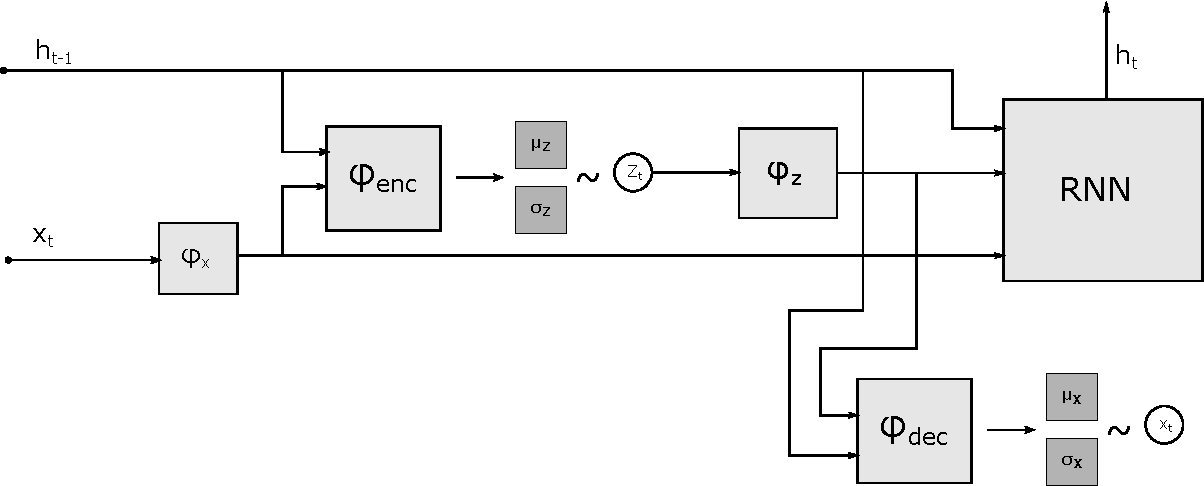
\includegraphics[width=0.9\textwidth]{figures/rnnvae/Fig1.pdf}
  \caption{Building block of the network, for a single channel (channel label not included for clarity). $x_t$ is a time-step of the input sequence, and $h_t$ is a hidden state of the RNN. }\label{fig:rnn}
\end{figure}

\subsubsection{Derivation of the lower bound}
The optimization objective of our variational setting is the evidence lower bound (ELBO) \cite{Kingma2014} on the log likelihood of the data. We can define it as:

\begin{equation} 
\begin{aligned}
\displaystyle
    \ln \mathit{p}(x_{\leq T}) &= \mathbb{E}_c \int \mathit{q}(z_{\leq T}|x^c_{\leq T}) \ln \mathit{p}(x^c_{\leq T}) \,dz_{\leq T}, \\
&= \mathbb{E}_c \int \mathit{q}(z_{\leq T}|x^c_{\leq T}) \ln \left( \frac{\mathit{p}(z_{\leq T},x^c_{\leq T})}{\mathit{p}(z_{\leq T}|x^c_{\leq T})} \right) \,dz_{\leq T},
\end{aligned} \label{rnn:eq_loglike}
\end{equation}

, over all channels $C$ and timepoints $T$. From the previous expression, $\mathit{p}(z_{\leq T}|x_{\leq T})$ is intractable. We can decompose it by factoring the numerator, in a similar way as Equation \ref{eq:decfact}:

\begin{equation} 
\begin{aligned}
\displaystyle
= \mathbb{E}_c \int \mathit{q}(z_{\leq T}|x^c_{\leq T}) \ln \left( \prod^T_{t=1} \frac{\mathit{p}(z_t |x^c_{< T}, z_{< T})\mathit{p}(x^c_t |z_{\leq t}, x_{< t})}{\mathit{q}(z_t |x^c_{\leq t}, z_{< t})} \right) \,dz_{\leq T}
\end{aligned}
\end{equation}

\begin{equation} 
\begin{aligned}
\displaystyle
= \mathbb{E}_c \int \sum^T_{t=1} \mathit{q}(z_{\leq T}|x^c_{\leq T}) \ln \left( \frac{\mathit{p}(z_t |x^c_{< t}, z_{< t})\mathit{p}(x^c_t |z_{\leq t}, x^c_{< t})}{\mathit{q}(z_t |x^c_{\leq t}, z_{< t})} \right) \,dz_{\leq T}
\end{aligned}
\end{equation}

\begin{equation} 
\begin{aligned}
\displaystyle
= \mathbb{E}_c \sum^T_{t=1} \int \mathit{q}(z_{\leq T}|x^c_{\leq T}) \ln \left( \frac{\mathit{p}(z_t |x^c_{< t}, z_{< t})\mathit{p}(x^c_t |z_{\leq t}, x^c_{< t})}{\mathit{q}(z_t |x^c_{\leq t}, z_{< t})} \right)\, dz_{\leq t}
\end{aligned}
\end{equation}

We decompose the inner expression:
%% \mathit{q}(z_{\leq t}|x_{\leq t}) = \mathit{q}(z_t|x_{\leq t}, z_{\lt t}) q(z_{\lt t} | x_{\lt t} ) 

\begin{equation} 
\begin{aligned}
\displaystyle
= \mathbb{E}_c \sum^T_{t=1} & \int \mathit{q}(z_{\leq t}|x^c_{\leq t}) \ln \mathit{p}(x^c_t |z_{\leq T}, x^c_{< t}) dz_{\leq t} \\
&- \int \mathit{q}(z_{< t}|x^c_{< t}) \ln \frac{\mathit{p}(z_t |x^c_{< t}, z_{< t})}{\mathit{q}(z_t |x^c_{\leq t}, z_{< t})} \,dz_{< t}
\end{aligned}
\end{equation}

The second term is the KL divergence between the real and approximate posterior:

\begin{equation} 
\begin{aligned}
\displaystyle
= \mathbb{E}_c \sum^T_{t=1}  & \int \mathit{q}(z_{\leq t}|x^c_{\leq t}) + \mathit{p}(x^c_t |z_{\leq T}, x^c_{< t}) dz_{\leq t} \\
- & \int \mathit{q}(z_{< t}|x^c_{< t}) \mathcal{D}_{KL}(\mathit{q}(z_t |x^c_{\leq t}, z_{< t}) || \mathit{p}(z_t |x^c_{< t}, z_{< t})) \,dz_{< t}
\end{aligned}
\end{equation}

Which finally leads to:

\begin{equation} 
\begin{aligned}
\displaystyle
= \mathbb{E}_c \,\mathbb{E}_{\mathit{q}(z_{\leq T}|x^c_{\leq T})}  \Big[ & \sum^T_{t=1} \ln \mathit{p}(x^c_t |z_{\leq T}, x^c_{< t}) \\
&- \mathcal{D}_{KL}(\mathit{q}(z_t |x^c_{\leq t}, z_{< t}) || \mathit{p}(z_t |x^c_{< t}, z_{< t})) \Big]
\end{aligned}
\end{equation}

As the channels are conditionally independent from the others, we can factorize the log likelihood  over each individual channel as:

\begin{equation} 
\begin{aligned} \label{rnn:eq:finalopt}
\displaystyle
= \mathbb{E}_c \,\mathbb{E}_{\mathit{q}(z_{\leq T}|x^c_{\leq T})}  \Big[ \sum^T_{t=1} & [ \sum^C_{i=1} \ln \mathit{p}(x^i_t |z_{\leq T}, x^i_{< t}) ] \\
&- \mathcal{D}_{KL}( \mathit{q}(z_t |x^c_{\leq t}, z_{< t}) || \mathit{p}(z_t |x_{< t}, z_{< t})) \Big]
\end{aligned}
\end{equation}

And, given that $\mathcal{D}_{KL}$ is non-negative, the first term of the expression is the lower bound of the log likelihood, with the $\mathcal{D}_{KL}$ being the gap between both expressions. Thus, by maximizing this lower bound with respect to the model parameters, we are also minimizing the log likelihood in equation \ref{rnn:eq_loglike}. The first term of Equation \ref{rnn:eq:finalopt} forces a joint decoding of the channels at each time point, allowing us to predict missing channels at any time point. The second term, which acts as regularization, forces the encoders of each channel to be close to a common prior generated from the previous time-point, enforcing a temporal structure.

\subsubsection{Channel reconstruction}

As previously mentioned, thanks to the first term of the lower bound in Equation \ref{rnn:eq:finalopt}, we are able to reconstruct data for a missing channel using existing ones. For a missing channel $c_{m}$, and for each timepoint $t$, we decode the associated latent space $z$ of each existing channel, and reconstruct the missing channel:

\begin{equation}
    x^{c_m}_t = \mathbb{E}_{c} [ \mathbb{E}_{q(z|x^c_t)} \sum p(x^m_t|z) ],
\end{equation}

%% AIXÒ MENCIONAR-HO A LA REUNIÓ per VEURE que podem FER
% \subsubsection{Joint prior optimization} \label{rnn:subsubsec:joinprior}
% For the optimization of Equation \ref{rnn:eq:finalopt}, we need to define the prior at each time % point (Equation \ref{rnn:eq:prior}). We explore two different expressions of the common prior:

% \begin{itemize}
%     \item $z_t \sim \varphi_{prior}(h^c_{t-1})$. We make the assumption that the prior will define the same latent space $z$, but does not directly enforce it.
%     \item $z_t \sim\varphi_{prior} (1/C \sum^C h^c_{t-1})$. We average the hidden state of each channel and obtain a single prior.
%     \item $z_t \sim 1/C \sum^C \varphi_{prior}(h^c_{t-1})$. This averages the output distributions of each channel on a single distribution, which is assumed to be the actual prior.
% \end{itemize}

\subsubsection{Variational dropout} 

Variational dropout was proposed by Kingma et al. \cite{Kingma2015} to regularize variational autoencoders and sparsify their latent space, by specifying a reparametrization of the posterior and learning the dropout rates of each latent dimension via a trainable parameter. Variational dropout requires a reparametrization on the encoder:

\begin{equation}
    \mathti{q}(z_t | x^c_{\leq t}, z_{\lt t}) \sim \mathcal{N}(\alpha\mu_{z,t},\alpha^2),
\end{equation}

with $\alpha$ being a learned parameter shared across channels and time-points. With this reparametrization, we can use an approximation of $\mathcal{D}_{KL}$, defined on \cite{Kingma2015}, that only depends on $\varalpha$. This approximation, however, requires the prior to be log-scale uniform. As in our model we have a defined prior for $t>0$ (Equation \ref{rnn:eq:prior}), this assumption only holds when $t=0$. We experimented with applying this reparametrization and only approximating $\mathcal{D}_{KL}$ for $t=0$. We conducted a number of synthetic and real data experiments to assess the effect of this approach.

\subsubsection{Missing data and variable number of time-points}

The described method works when $T$ is the same across channels, and when there are no missing data points. However, with real data, that is not always the case. To account for missing data, for each timepoint $t$, we limit our summation over samples that have that time-point, and we do the same for missing channels. However, this could lead to a bias towards samples with more timepoints. For this reason, we add a mean term for each subject to both terms of the loss, to make every subject weight equally regardless of their number of timepoints. \\

In the case where a channel only has a time point (e.g. demographic data, or genetic information, which is not longitudinal), the channel is only included on the loss when $t=0$, and is considered as a channel with only one time-point for all the related calculations.

\subsection{Data}

Experiments on the method were performed on both synthetic and real data. In this section, we describe their characteristics.

\subsubsection{Synthetic data}

We generated multi-channel synthetic temporal data. We implemented a generation method of longitudinal data from a set of latent variables of a fixed dimensionality. We generated the data using the following expression:

\begin{equation} 
\begin{gathered} \label{rnn:eq:synthdata}
   z \sim \mathbb{N}(0, I_{l}) \\
   \varepsilon \sim \mathbb{N}(0, 1) \\
   x^c_t = W^{c}z + f_{long}(t) + \varepsilon
\end{gathered}
\end{equation}

$I_{l}$ is the identity matrix with size $l \times l$, where $l$ is the latent space size. $W^c \in \mathbb{R}^{g \times l}$, with $g$ being the number of features of the output channel, is a random orthonormal matrix that linearly relates each channel $c$ to the latent space.  $f_{long}$ represents the temporal component of the data, depending on time-point $t$, and $\varepsilon$ is a random noise variable. \\

Each channel will have a different longitudinal component, depending on a common underlying latent space. We will test the performance of variational dropout for different values of $l$. We will also visually assess if the network is able to reconstruct the original channel. For the $f_{long}$ function, we use basic sigmoid, cosinus and sinus functions.   \\

%%% FIGURE WHERE i put each TRAJECTORY AND POINTS
%\begin{figure}[!htbp]
%  \centering
%  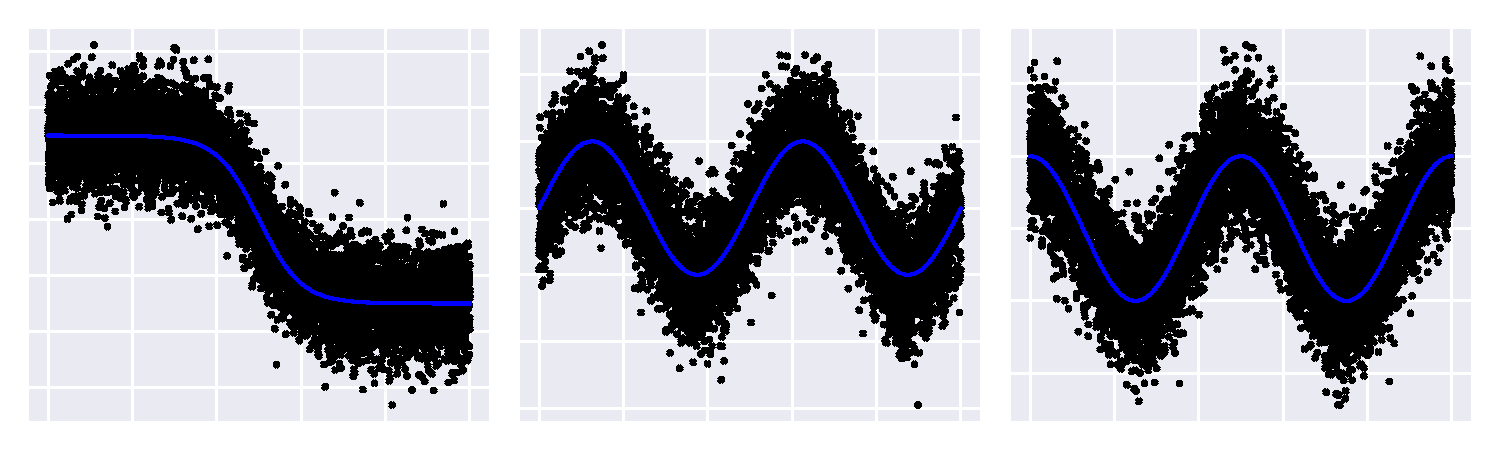
\includegraphics[width=0.9\textwidth]{figures/rnnvae/samples_long_2.pdf}
%  \caption{Functions used for the temporal component of the synthetic data. Function in blue, cloud %of samples taken (with noise) in black. From left to right: sigmoid, cosinus and sinus %functions.}\label{fig:rnn:synth1}
%\end{figure}

\subsubsection{ADNI data}

Data used in this chapter were obtained from the Alzheimer’s Disease Neuroimaging Initiative (ADNI) database \cite{Mueller2005}. The ADNI was launched in 2003 as a public-private partnership, led by Principal Investigator Michael W. Weiner, MD. The primary goal of ADNI has been to test whether serial biological imaging markers, and clinical and neuropsychological assessment can be combined to measure the progression of MCI and early AD. \\

We focused on five different data modalities. Full relation of features used can be found in supplementary file S1: \\

\begin{itemize}
    \item Brain subcortical volumes: We select MRI T1 weighted images, preprocessed using gradient warping, scaling, B1 correction and N3 homogeneity correction. Images were then automatically processed with the longitudinal pipeline \cite{Reuter2012} in FreeSurfer. Specifically, an unbiased within-subject template space and image is created using robust, inverse consistent registration \cite{Reuter2010}. Several processing steps, such as skull stripping, Talairach transforms, atlas registration as well as spherical surface maps and parcellations are then initialized with common information from the within-subject template, significantly increasing reliability and statistical power. We use the parcelled subcortical volumes, obtaining 40 features.
    \item Cortical thickness: We use the same imaging pipeline described above. We use the parcelled cortical thickness, obtaining 68 features.
    \item Cognitive assessment scores: A set of six different neuropsychological assessment tests that capture the level of cognitive decline of the patients in specific tasks and domains. 
    \item Demographic information: three features of main demographic information age, sex and years of education of the patient. This is a cross-sectional, baseline only modality.
    \item APOE (Apolipoprotein) $\varepsilon4$ allele load: a single feature indicating the number of copies of this allele, which is a risk factor of AD \cite{Saunders1993}. This is a cross-sectional, baseline only modality.
\end{itemize}

We selected subjects that had no missing data at their baseline acquisition for any of the channels, and all subsequent follow-ups that had, at least, one of the existing longitudinal modalities, and had no missing features intra-modality. With this criteria, we selected 897 subjects, with a total of 7224 acquisitions. Table \ref{rnn:demographic} show the demographic information of the selected cohort. Regarding the distribution of the data across modalities, Figure \ref{fig:rnn:missingdata} shows the information about missing, mean and maximum number of acquisitions across modalities.

\begin{table}[!htbp]
\centering
\begin{tabular}{@{}ccccc@{}}
\toprule
          & CN & MCI & AD & Total \\ \midrule
Nº scans  & 229          & 324    & 180 & 897   \\
Age       & $74.62\pm5.26$ & $73.70\pm7.33$ & $73.66\pm7.84$  &  $73.57\pm6.92$     \\
Education & $16.23\pm2.72$ & $15.67\pm2.98$ & $14.95\pm2.93$  &  $15.77\pm2.88$     \\
MMSE      & $29.06\pm1.09$ & $27.13\pm1.80$ & $23.19\pm1.97$  & $27.09\pm2.65$      \\
Female    &  $51.53 \%$   & $40.12 \%$      &  $50.55\%$      &  $46.7\%$    \\
APOE      & $27.51\%$    & $56.17\%$        & $51.1\%$        & $47.8\%$     \\ \bottomrule
\end{tabular}
\caption[Demographic characteristics of the cohort used, at baseline.]{Demographic characteristics of the cohort at baseline. Age and education presented as average and standard deviation, in years. APOE4: Apolipoprotein $\varepsilon$4, percentage with 1 or 2 alleles. CN: Cognitively normal. MCI: Mild cognitive impairment. AD: Alzheimer’s disease. MMSE: Mini-mental state examination. }\label{rnn:demographic}
\end{table}

\begin{figure}[!htbp]
  \centering
  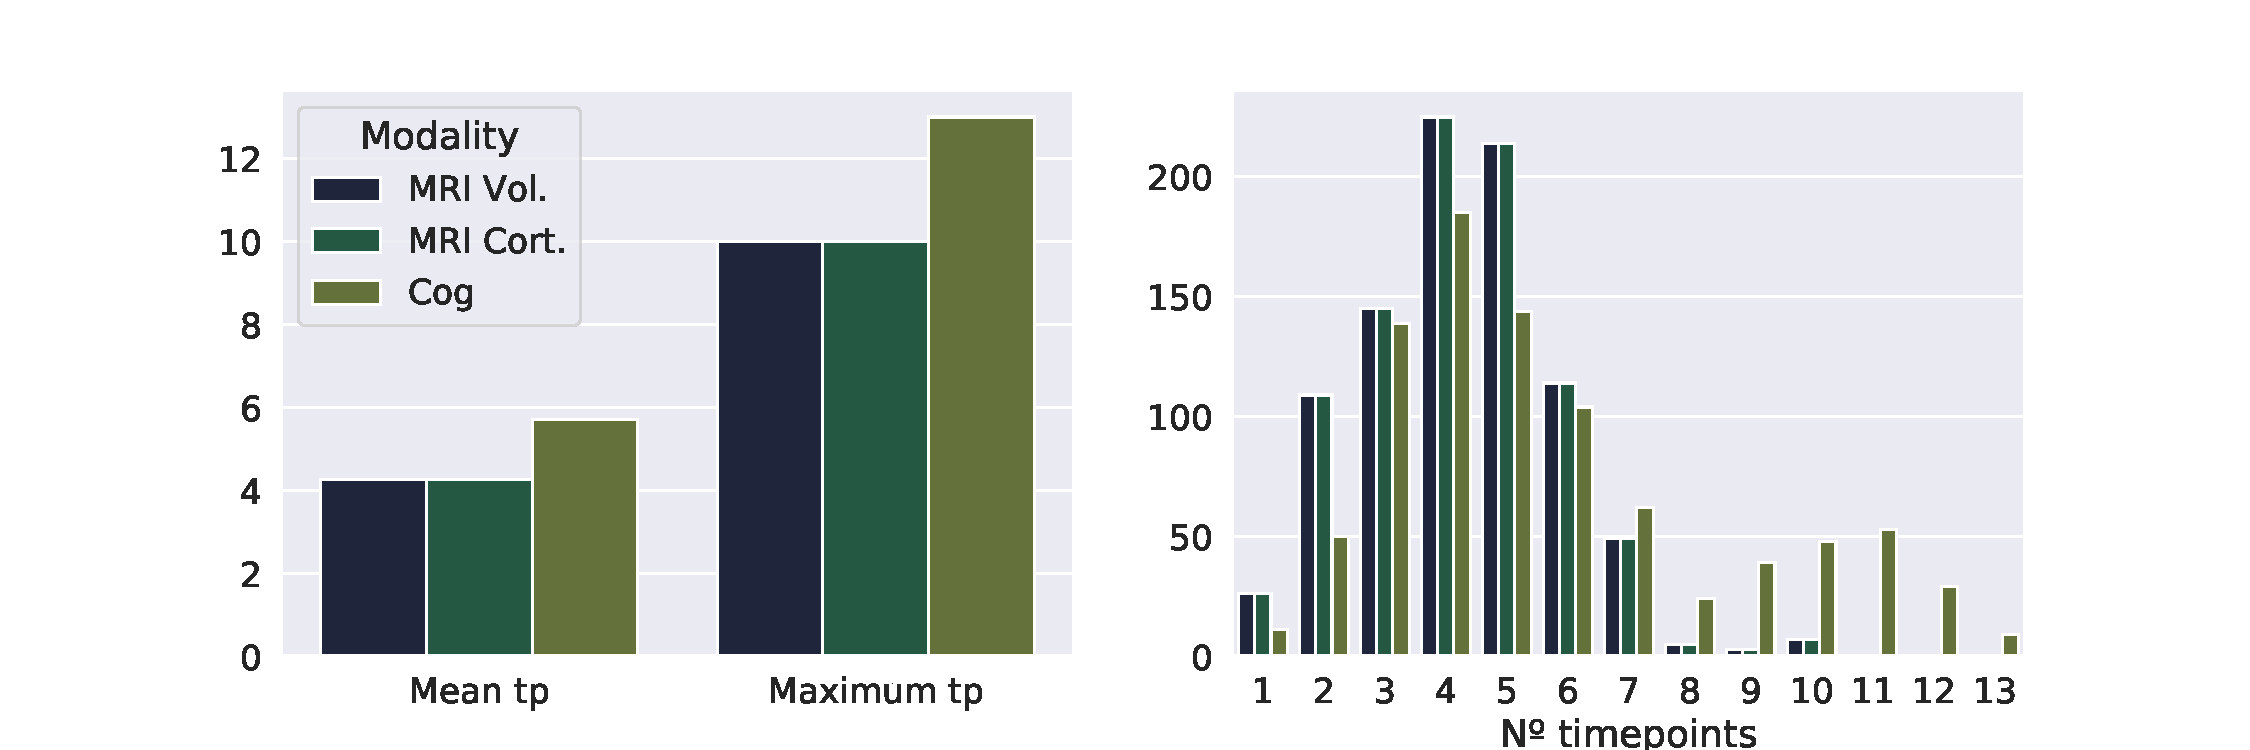
\includegraphics[width=1.0\textwidth]{figures/rnnvae/rnn_long.pdf}
  \caption[Time point distribution of ADNI data.]{Left: mean and maximum amount of time points for the three longitudinal channels. Right: distribution of sequence length across subjects, for each longitudinal channel.}\label{fig:rnn:missingdata}
\end{figure}

Other relevant modalities were considered, such as PET derived biomarkers or CSF fluid information, but were ultimately not included due to their low amount of subjects with acquisitions available and low number of follow-ups. \\ 

\subsection{Experiments}

Our experiments with synthetic data were aimed at both showing that the model is able to reconstruct longitudinal signals from missing channels, and to test whether cross-sectional variational dropout would hold for our longitudinal implementation. The parameters used in this model are described in Table \ref{rnn:tablehyper} (first column). We tested for three different real latent dimensions ($l \in {5,10,15}$) and observe if the network is able to select a similar number of latent spaces after applying variational dropout. \\

For the ADNI cohort, we first separate our data between a train and a test set, with 90/10 separation, while maintaining proportion of diagnosis across sets. The test set is then held-out, and we perform an hyperparameter search on the train set using 10-fold cross validation over a predefined parameter space, described in Table \ref{rnn:tablehyper} (second column). \\

%%% ACTUALITZAR AL FINAL
\begin{table}[!htbp]
\centering
\begin{tabular}{@{}ccc@{}}
\toprule
Hyperparam & Synthetic model & ADNI model \\ \midrule
RNN hidden    &   20    & 100, 200, 300  \\
nº latent dim    &  15   & 10, 20, 30 \\
nº layers    &  1   & 0, 1  \\
hidden RNN size  &  30   & 100, 200, 300  \\ \bottomrule
\end{tabular}
\caption[Hyperparameter table.]{Table of hyperparameters. Left column: parameters used with the synthetic model. Right column: parameters used for ADNI model optimization.}\label{rnn:tablehyper}
\end{table}

Model is trained using gradient descent with Adam \cite{Kingma2015a}, at $1e-3$ learning rate, until convergence of the model (roughly 1500 epochs). Code and training settings of the model can be found in the repository of the chapter\footnote{https://github.com/GerardMJuan/RNN-VAE}. \\

We evaluate our results on the held-out test set on two different tasks: 

\begin{itemize}
    \item \textbf{Time-point prediction:} we remove the last time-point data from each subject in the test set, and we predict it using the rest of the data. 
    \item \textbf{Channel reconstruction:} we reconstruct each different channel from the rest of the channels, using the joint decoder $p_c(x|z)$. We evaluate the results using different combinations of channels.
\end{itemize}

For the first task, we compare the performance of our model to two baseline methods: constant, using as prediction the previous time-point data; and linear, doing a linear regression for each sample and channel to predict the missing time point. For the second task, we compare our method to a baseline method based on k-means: for each sample in the test set, we perform a k-means search for each individual channel to find the closest sample in our training set. For each of those samples, we select the channel we are reconstructing, and we average them to obtain the reconstructed channel for the original sample. We evaluate both tasks using mean absolute error (MAE). \\

%% Qualitative results? Generating from latent space and showing the generated data, or draw trajectories over the latent space.
We also test the generative capabilities of the model by reconstructing the cortical and subcortical data of two synthetic patients: one with a stable, healthy cognitive trajectory, and another one which is rapidly declining. We generate 4 time points for each of the subjects, and visualize the longitudinal neurodegeneration trajectories and their plausability. Information about the exact data used for those synthetic patients can be found in Supplementary data S2. \\

\section{Results}
\label{rnn:results}

\subsection{Synthetic results}

We generated 500 samples, with $g=20$, and using three channels, each with a different longitudinal trajectory. Figure \ref{fig:rnn:synth1} shows the reconstruction of the three channels, using all channels (top row) and witholding the original channel and reconstructing from the other two (bottom row). 

\begin{figure}[!htbp]
  \centering
  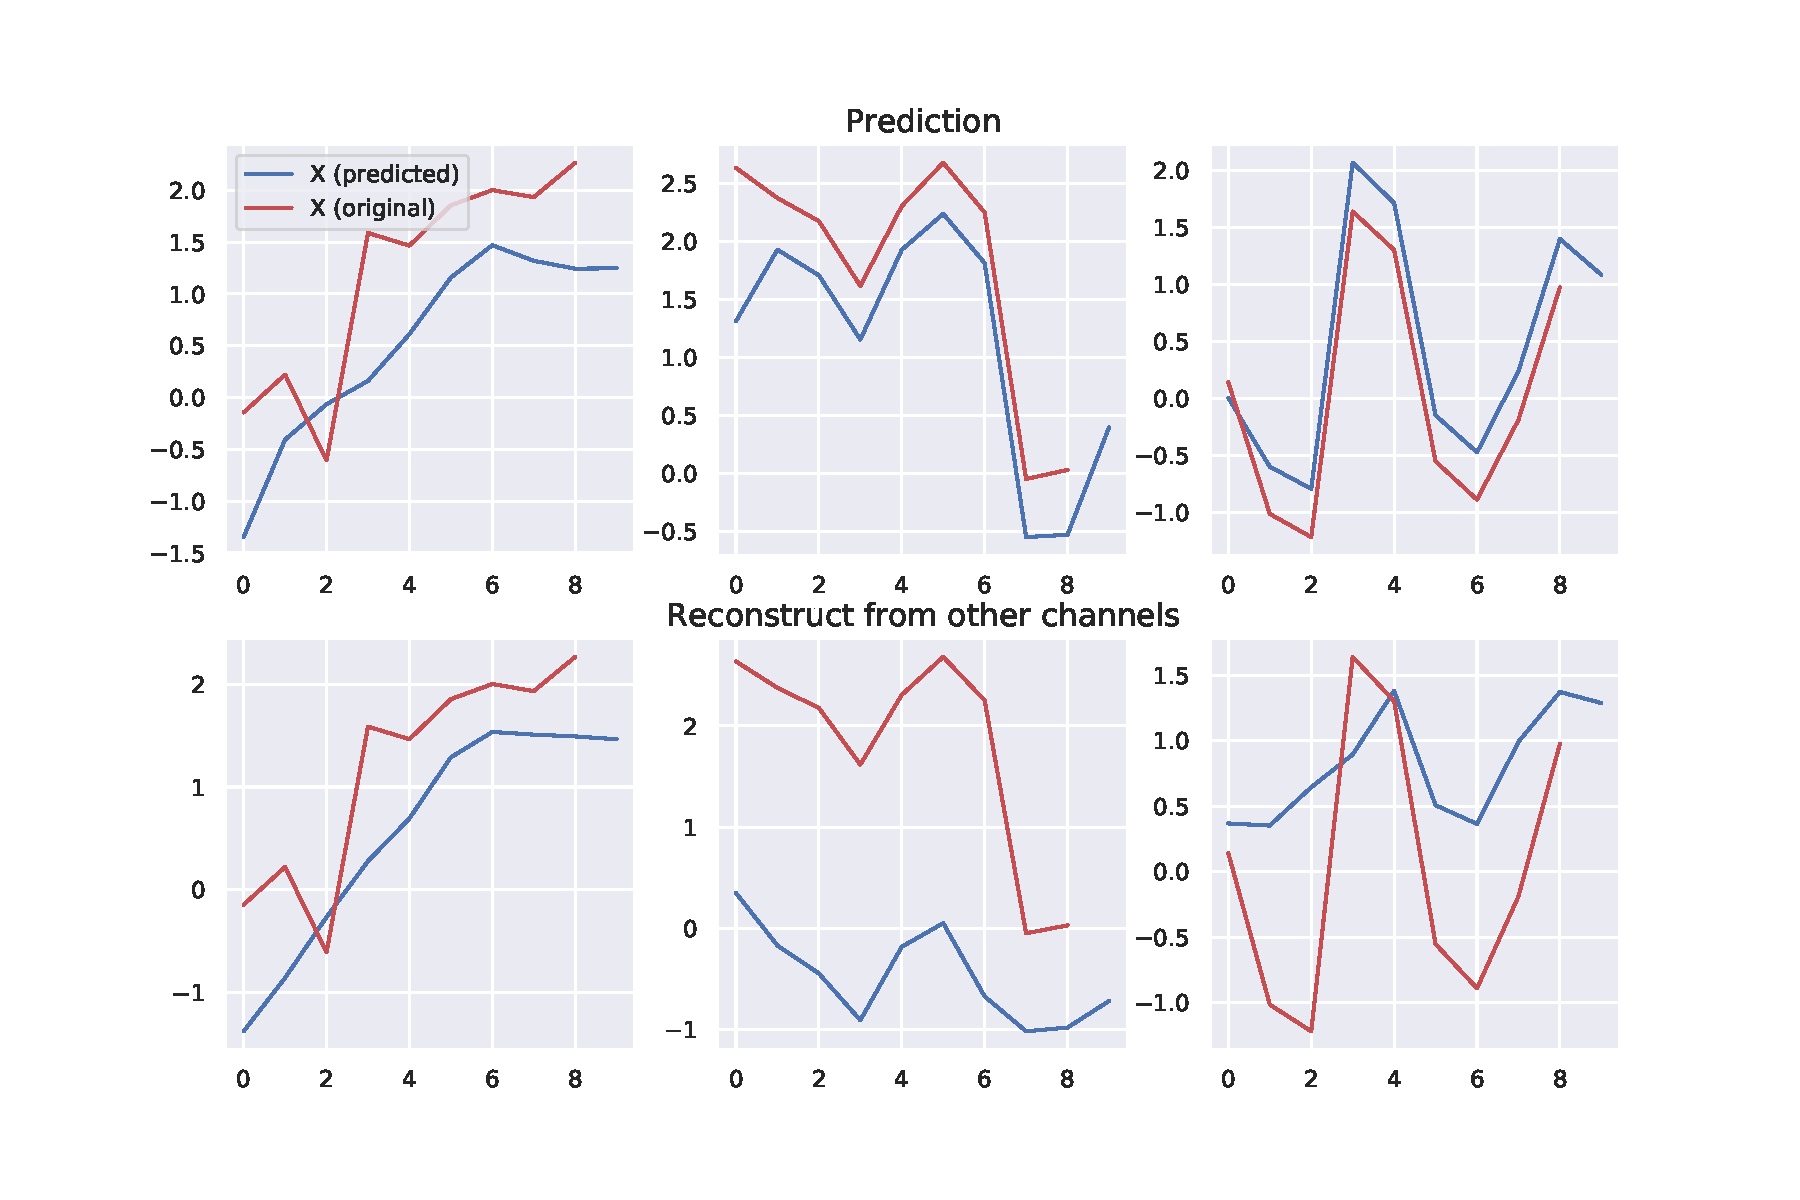
\includegraphics[width=1.0\textwidth]{figures/rnnvae/synth_recon.pdf}
  \caption[Synthetic data reconstruction.]{Reconstruction of the three channels of the generated synthetic data. Top row: reconstruction using all the channels. Bottom row: reconstruction using the other two channels.}\label{fig:rnn:synth2}
\end{figure}

\begin{figure}[!htbp]
  \centering
  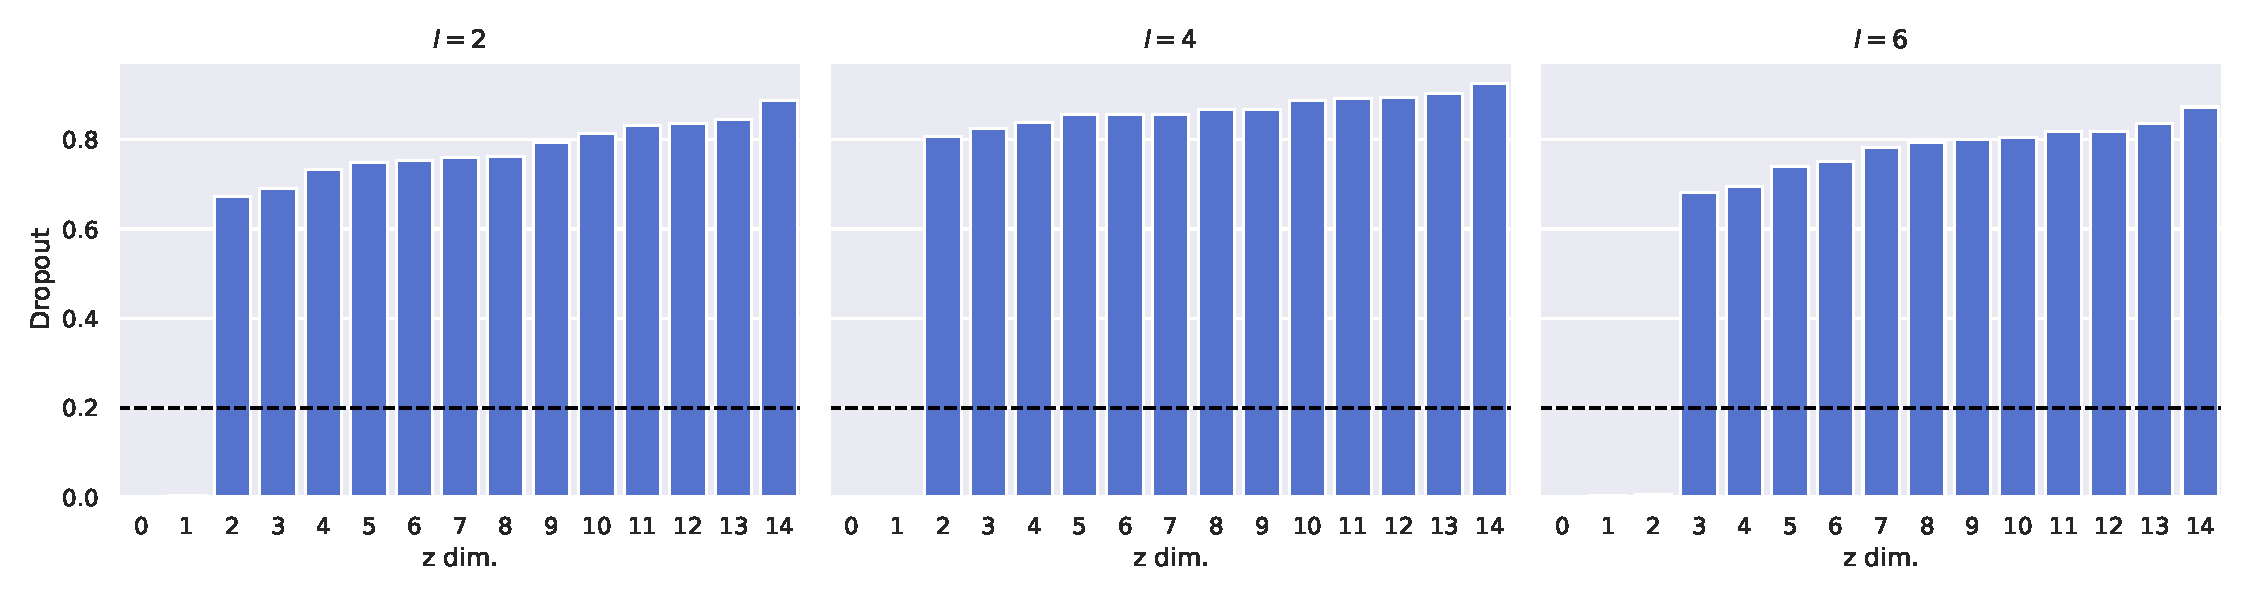
\includegraphics[width=1.0\textwidth]{figures/rnnvae/synthvardrop.pdf}
  \caption[Variational dropout.]{Variational dropout for each latent space dimension of the model, for three different real latent spaces.}\label{fig:rnn:synthvar}
\end{figure}

Regarding the application of variational dropout, Figure \ref{fig:rnn:synth2} shows the dropout after generating data with different true latent dimensions, compared to the actual latent dimensions of the data.

\subsection{ADNI results}

After hyperparameter optimization, we selected ${Rnn hidden=300, lat_dim = 20, n_layers = 1 and hidden RNN size=300}$ as the best parameters. Table \ref{fig:results:data} shows the results in the two tasks described, on the hold-out test set, and comparing it to the baseline models described above. We show results for single channel and multi-channel networks.

\begin{table}[!htbp]
\centering
\resizebox{0.95\textwidth}{!}{%
\begin{tabular}{@{}ccccccccc@{}}
\toprule
             & \multicolumn{3}{c}{Long. prediction} & \multicolumn{5}{c}{Channel rec.}      \\ \midrule
             & MRI (vol.)   & MRI (cort.)   & Cog.  & MRI (vol.) & MRI (cort.) & Cog. & Demog. & APOE \\ \midrule
%Constant     &  0.215  &  0.349   &  0.438     & -          & -           & -    & -      & -    \\
Linear       &  0.240  &  0.395   &  0.486     & -          & -           & -    & -      & -    \\
KNN          & -       & -  & -     &  0.789   &    0.77  & 0.703     & 1.005       &     0.901 \\
RVAE      &  0.235  & 0.359  &  0.451  &   -  &     -       & -    &   -    &   -  \\
MC-RVAE &     0.405    &  0.561  & 0.647 &  0.691   &  0.689    &  0.619    &   0.847 & 0.885 \\ \bottomrule
\end{tabular}}
\caption[Performance of the model.]{Performance of the models on longitudinal prediction and channel reconstruction, compared to baseline methods. RNN-VAE: single channel model.  MC-RVAE: multiple channel model. All values are mean absolute error (MAE) over each subject and time-point.} \label{table:results:data}
\end{table}

Figure \ref{fig:rnn:latent} show the latent space on the test set colored by diagnosis and by timepoint. \\

\begin{figure}[!htbp]
  \centering
  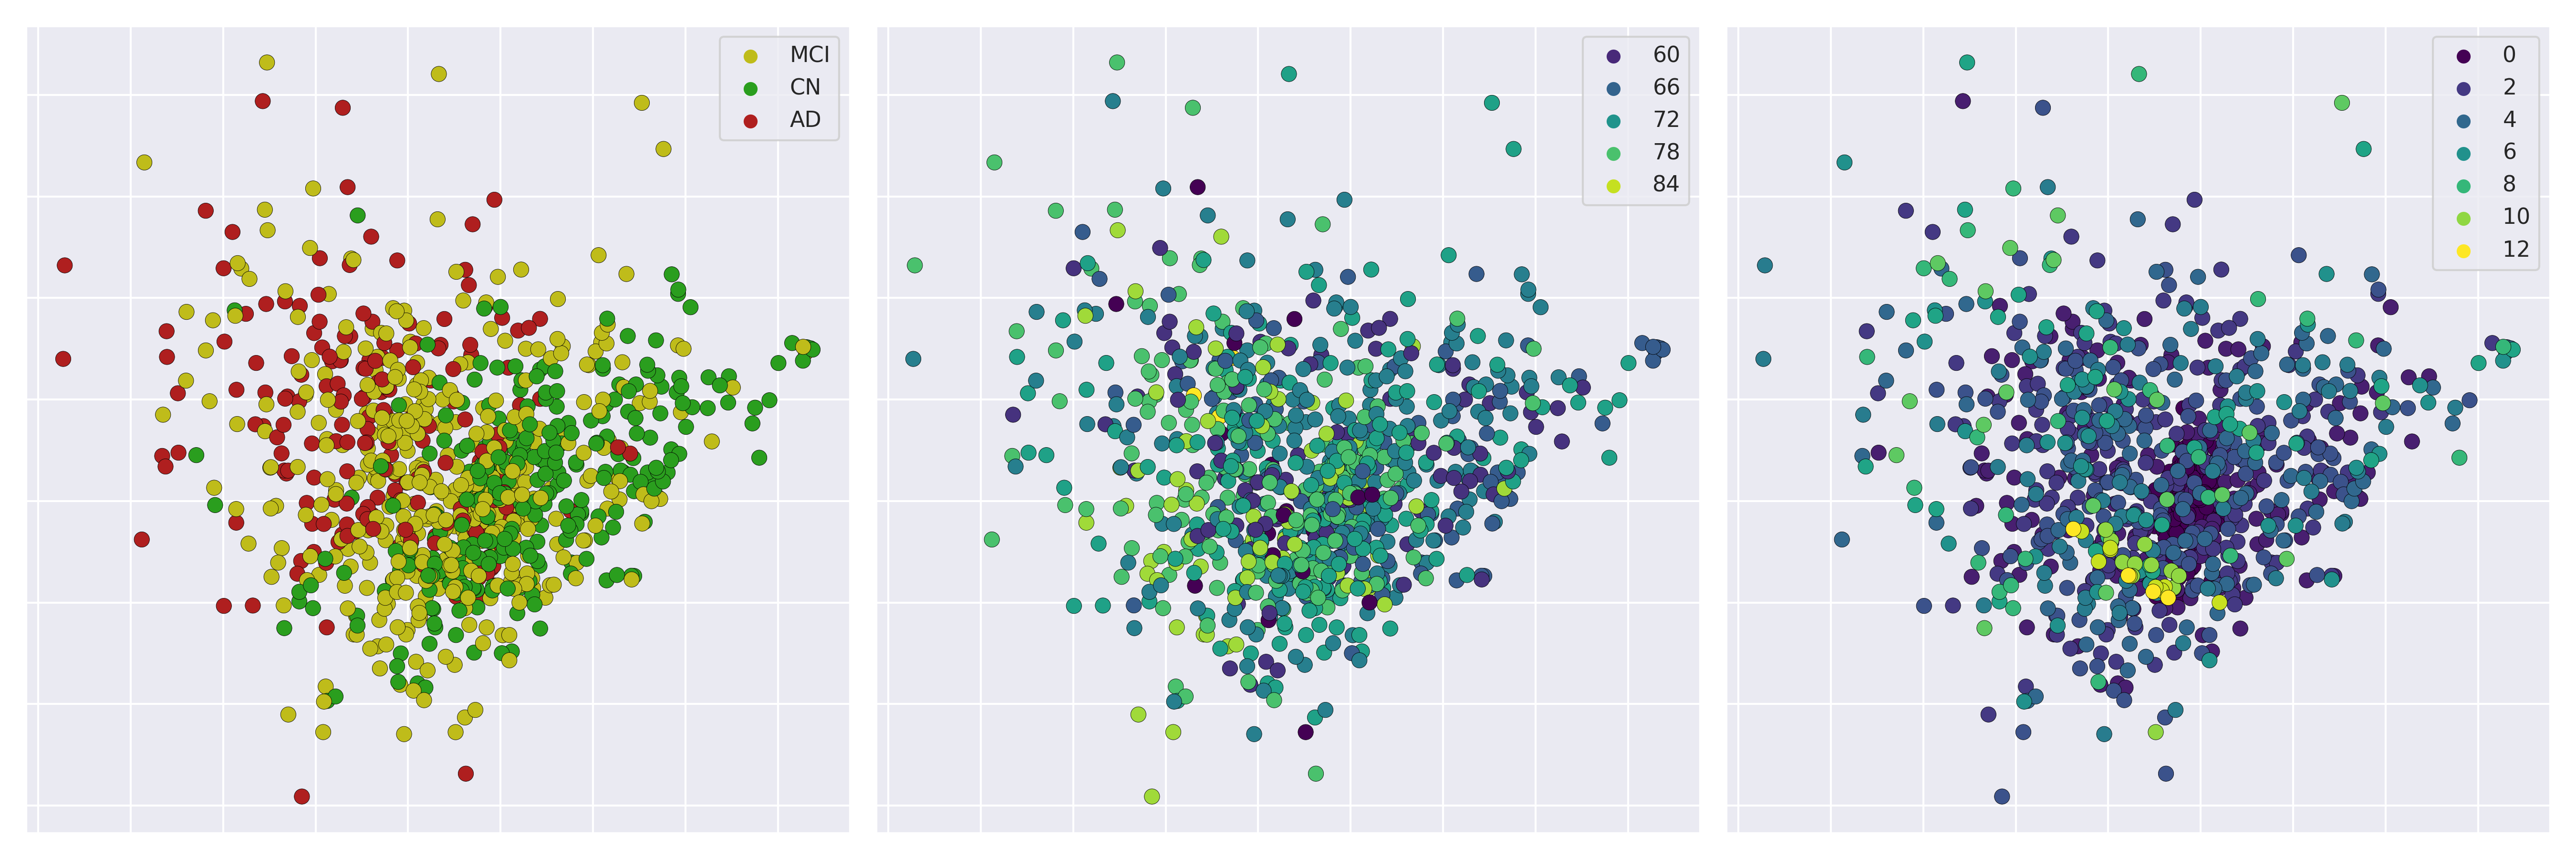
\includegraphics[width=1.0\textwidth]{figures/rnnvae/latent_space_fig.png}
  \caption[Latent space for the test set.]{Dimensions 0 and 1 of the latent space, for subjects on the hold-out test set. Each point represents a different time-point. Left graphic: colored by diagnosis. Middle: colored by age. Right: colored by time-point.}\label{fig:rnn:latent}
\end{figure}

%% IF TIME: SHOW DIFFERENCE IN DECLINING USING APOE=0 AND APOE=2. THIS IS AN EXTRA FIGURE
Figure \ref{fig:rnn:qualitative} show four synthetic timepoints of cortical and subcortical data. We sampled them using two sequences of 4 cognitive acquisitions: a typical sequence of healthy control, and a sequence of a rapidly declining patient, with similar demographic information.  Figures were generated using Brainpainter \cite{Marinescu2019a} \\

\begin{figure}[!htbp]
  \centering
  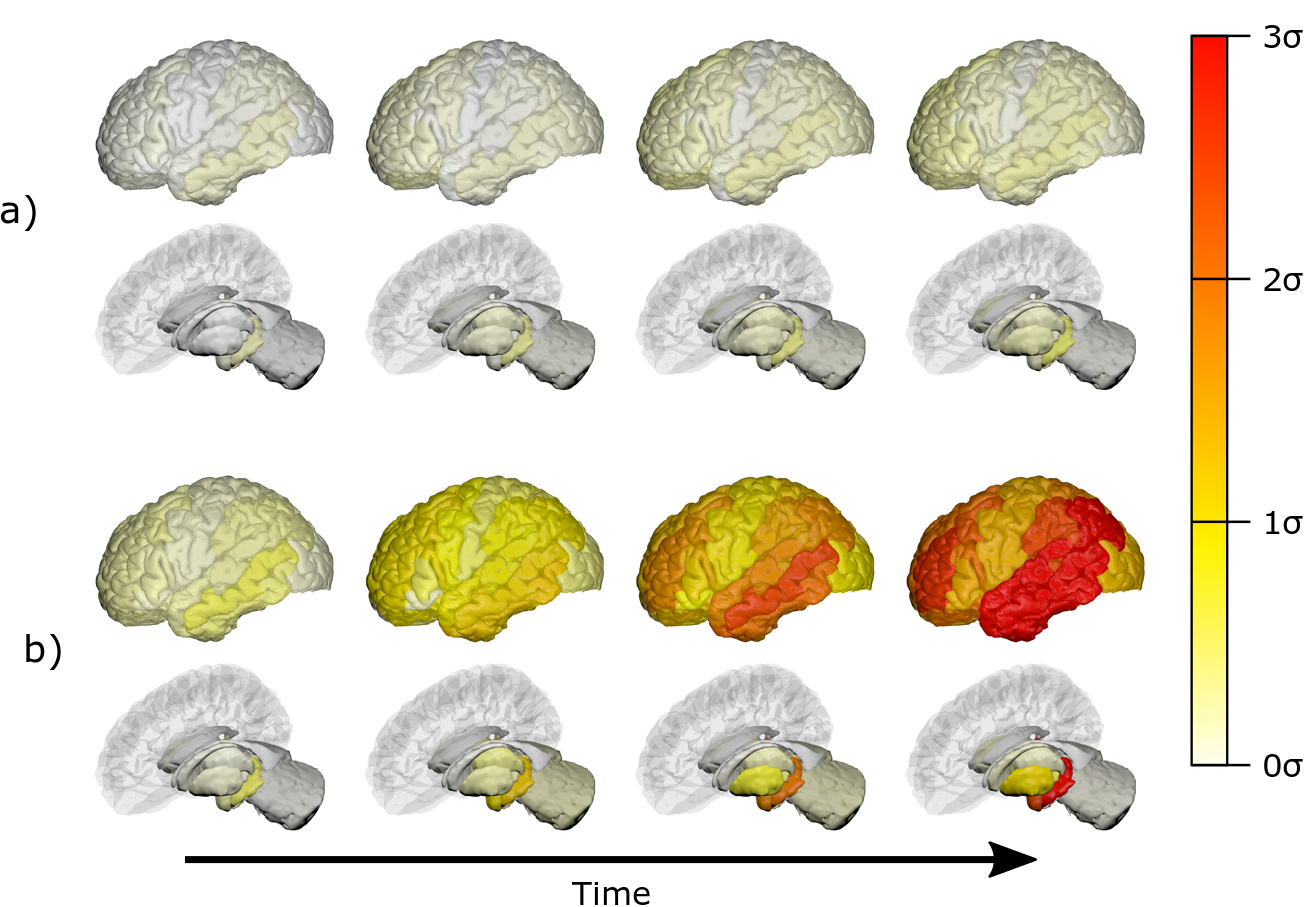
\includegraphics[width=1.0\textwidth]{figures/rnnvae/brainpainter.png}
  \caption[Generated MRI-derived longitudinal markers.]{Trajectories of synthetic cortical and subcortical generated by RNN-MCVAE. $\sigma$: standard deviation of the control population. a) and b) corresponds to the patients described in the main text.}
 \label{fig:rnn:qualitative}
\end{figure}

\section{Discussion}
\label{rnn:discussion}

% Introducció curta del paper.
In this chapter we proposed a generative method based on recurrent variational autoencoders that is able to jointly model a latent trajectory from multimodal data. We introduced the main concepts and assumptions behind the model, derived its lower bound, and tested it both on synthetic and real data from a cohort of patients afflicted by AD. \\

% able to multimodal data
% able to bla bla bla 
In our synthetic tests, we showed the strength of the method for reconstructing longitduinal signals (Figure \ref{fig:rnn:synth2}). Even in the cases where no information about the original channel is fed to the model, it is still able to reconstruct the general trajectory of the signal by using information from other channels (Figure \ref{fig:rnn:synth2}, bottom row). However, the effect of variational dropout in our model is still not clear, as we show in Figure \ref{fig:rnn:synthvar}. The number of latent dimensions selected stays constant along real latent dimensions. Variational dropout for our model needs to be further addressed and adapted to the temporal structure of the latent space, and we have decided not to use it on the tests using the ADNI cohort until more testing is carried out.  \\

For the ADNI cohort, we compared the performance of our model on reconstructing each channel from the others, and on predicting the next time-point. Table \ref{table:results:data} shows the results for using a single channel model for each modality, and using the joint model. Performance on prediction seems to suffer, while we manage to obtain a good reconstruction compared to baseline. Performance could likely be improved by further hyperparameter and model exploration. Visualization of the latent space generated in the joint model, shown in Figure \ref{fig:rnn:latent}, shows the distribution of the latent codes of each subject by DX, age and tp, for selected dimensions. While we can observe a good separation between diagnosis and age, we do not appreciate a distinct temporal structure.  \\

To demonstrate the reconstruction capability of the model, Figure \ref{fig:rnn:qualitative} shows two different sequences of cortical and subcortical MRI data generated by the network, for a cognitive healthy patient and a rapidly declining patient. The generated data present a plausible decline of cortical thickness for both cases. \\

% Comparació amb d'altres papers? com enfoquen les discussions?
Compared to existing methods, our model principal contribution is its flexibility to scale to larger number of channels and variable number of time-points. Cao et al. \cite{Cao2019} model, which is based on canonical correlation analysis, can only use two different longitudinal channels, and it is not a generative model. Compared to the multi-channel model of Antelmi et al. \cite{Antelmi2019}, from which our model is build upon, our implementation includes temporal structure and allows for temporal data to be included and generated. \\

\section{Conclusions}
\label{rnn:conclusions}

% put some of the info from the real conclusions here
We developed and tested a generative model on multimodal, longitudinal data based on recurrent variational autoencoders. The model is able to combine different modalities of variable length longitudinal data, predict future data, and reconstruct missing modalities. Current results show that the model has potential for missing data reconstruction and prediction tasks. The model performance and architecture, however, requires further development and testing, which is currently underway. Implementing variational dropout adapted to the temporal structure to the latent space would regularize the method and improve both interpretability and performance. We should also test the robustness of our model to predict more that one time-point, or how the performance changes with larger rates of missing data at each time-point. Another hindrance of our model is that we assume equal time between acquisitions, and we simplify sequences to not have any missing acquisitions alongside them. Using this information could lead to the ability to sample synthetic data at specific future points, which could be of use for clinical trial design. Finally, we should take advantage of the uncertainty learnt by the model to understand for which tasks and situations the model has less confidence, and improve on it.  \\